\documentclass{article} % For LaTeX2e
\usepackage{iclr2022_conference,times}
% Optional math commands from https://github.com/goodfeli/dlbook_notation.
%%%%% NEW MATH DEFINITIONS %%%%%

\usepackage{amsmath,amsfonts,bm}

% Mark sections of captions for referring to divisions of figures
\newcommand{\figleft}{{\em (Left)}}
\newcommand{\figcenter}{{\em (Center)}}
\newcommand{\figright}{{\em (Right)}}
\newcommand{\figtop}{{\em (Top)}}
\newcommand{\figbottom}{{\em (Bottom)}}
\newcommand{\captiona}{{\em (a)}}
\newcommand{\captionb}{{\em (b)}}
\newcommand{\captionc}{{\em (c)}}
\newcommand{\captiond}{{\em (d)}}

% Highlight a newly defined term
\newcommand{\newterm}[1]{{\bf #1}}


% Figure reference, lower-case.
\def\figref#1{figure~\ref{#1}}
% Figure reference, capital. For start of sentence
\def\Figref#1{Figure~\ref{#1}}
\def\twofigref#1#2{figures \ref{#1} and \ref{#2}}
\def\quadfigref#1#2#3#4{figures \ref{#1}, \ref{#2}, \ref{#3} and \ref{#4}}
% Section reference, lower-case.
\def\secref#1{section~\ref{#1}}
% Section reference, capital.
\def\Secref#1{Section~\ref{#1}}
% Reference to two sections.
\def\twosecrefs#1#2{sections \ref{#1} and \ref{#2}}
% Reference to three sections.
\def\secrefs#1#2#3{sections \ref{#1}, \ref{#2} and \ref{#3}}
% Reference to an equation, lower-case.
\def\eqref#1{equation~\ref{#1}}
% Reference to an equation, upper case
\def\Eqref#1{Equation~\ref{#1}}
% A raw reference to an equation---avoid using if possible
\def\plaineqref#1{\ref{#1}}
% Reference to a chapter, lower-case.
\def\chapref#1{chapter~\ref{#1}}
% Reference to an equation, upper case.
\def\Chapref#1{Chapter~\ref{#1}}
% Reference to a range of chapters
\def\rangechapref#1#2{chapters\ref{#1}--\ref{#2}}
% Reference to an algorithm, lower-case.
\def\algref#1{algorithm~\ref{#1}}
% Reference to an algorithm, upper case.
\def\Algref#1{Algorithm~\ref{#1}}
\def\twoalgref#1#2{algorithms \ref{#1} and \ref{#2}}
\def\Twoalgref#1#2{Algorithms \ref{#1} and \ref{#2}}
% Reference to a part, lower case
\def\partref#1{part~\ref{#1}}
% Reference to a part, upper case
\def\Partref#1{Part~\ref{#1}}
\def\twopartref#1#2{parts \ref{#1} and \ref{#2}}

\def\ceil#1{\lceil #1 \rceil}
\def\floor#1{\lfloor #1 \rfloor}
\def\1{\bm{1}}
\newcommand{\train}{\mathcal{D}}
\newcommand{\valid}{\mathcal{D_{\mathrm{valid}}}}
\newcommand{\test}{\mathcal{D_{\mathrm{test}}}}

\def\eps{{\epsilon}}


% Random variables
\def\reta{{\textnormal{$\eta$}}}
\def\ra{{\textnormal{a}}}
\def\rb{{\textnormal{b}}}
\def\rc{{\textnormal{c}}}
\def\rd{{\textnormal{d}}}
\def\re{{\textnormal{e}}}
\def\rf{{\textnormal{f}}}
\def\rg{{\textnormal{g}}}
\def\rh{{\textnormal{h}}}
\def\ri{{\textnormal{i}}}
\def\rj{{\textnormal{j}}}
\def\rk{{\textnormal{k}}}
\def\rl{{\textnormal{l}}}
% rm is already a command, just don't name any random variables m
\def\rn{{\textnormal{n}}}
\def\ro{{\textnormal{o}}}
\def\rp{{\textnormal{p}}}
\def\rq{{\textnormal{q}}}
\def\rr{{\textnormal{r}}}
\def\rs{{\textnormal{s}}}
\def\rt{{\textnormal{t}}}
\def\ru{{\textnormal{u}}}
\def\rv{{\textnormal{v}}}
\def\rw{{\textnormal{w}}}
\def\rx{{\textnormal{x}}}
\def\ry{{\textnormal{y}}}
\def\rz{{\textnormal{z}}}

% Random vectors
\def\rvepsilon{{\mathbf{\epsilon}}}
\def\rvtheta{{\mathbf{\theta}}}
\def\rva{{\mathbf{a}}}
\def\rvb{{\mathbf{b}}}
\def\rvc{{\mathbf{c}}}
\def\rvd{{\mathbf{d}}}
\def\rve{{\mathbf{e}}}
\def\rvf{{\mathbf{f}}}
\def\rvg{{\mathbf{g}}}
\def\rvh{{\mathbf{h}}}
\def\rvu{{\mathbf{i}}}
\def\rvj{{\mathbf{j}}}
\def\rvk{{\mathbf{k}}}
\def\rvl{{\mathbf{l}}}
\def\rvm{{\mathbf{m}}}
\def\rvn{{\mathbf{n}}}
\def\rvo{{\mathbf{o}}}
\def\rvp{{\mathbf{p}}}
\def\rvq{{\mathbf{q}}}
\def\rvr{{\mathbf{r}}}
\def\rvs{{\mathbf{s}}}
\def\rvt{{\mathbf{t}}}
\def\rvu{{\mathbf{u}}}
\def\rvv{{\mathbf{v}}}
\def\rvw{{\mathbf{w}}}
\def\rvx{{\mathbf{x}}}
\def\rvy{{\mathbf{y}}}
\def\rvz{{\mathbf{z}}}

% Elements of random vectors
\def\erva{{\textnormal{a}}}
\def\ervb{{\textnormal{b}}}
\def\ervc{{\textnormal{c}}}
\def\ervd{{\textnormal{d}}}
\def\erve{{\textnormal{e}}}
\def\ervf{{\textnormal{f}}}
\def\ervg{{\textnormal{g}}}
\def\ervh{{\textnormal{h}}}
\def\ervi{{\textnormal{i}}}
\def\ervj{{\textnormal{j}}}
\def\ervk{{\textnormal{k}}}
\def\ervl{{\textnormal{l}}}
\def\ervm{{\textnormal{m}}}
\def\ervn{{\textnormal{n}}}
\def\ervo{{\textnormal{o}}}
\def\ervp{{\textnormal{p}}}
\def\ervq{{\textnormal{q}}}
\def\ervr{{\textnormal{r}}}
\def\ervs{{\textnormal{s}}}
\def\ervt{{\textnormal{t}}}
\def\ervu{{\textnormal{u}}}
\def\ervv{{\textnormal{v}}}
\def\ervw{{\textnormal{w}}}
\def\ervx{{\textnormal{x}}}
\def\ervy{{\textnormal{y}}}
\def\ervz{{\textnormal{z}}}

% Random matrices
\def\rmA{{\mathbf{A}}}
\def\rmB{{\mathbf{B}}}
\def\rmC{{\mathbf{C}}}
\def\rmD{{\mathbf{D}}}
\def\rmE{{\mathbf{E}}}
\def\rmF{{\mathbf{F}}}
\def\rmG{{\mathbf{G}}}
\def\rmH{{\mathbf{H}}}
\def\rmI{{\mathbf{I}}}
\def\rmJ{{\mathbf{J}}}
\def\rmK{{\mathbf{K}}}
\def\rmL{{\mathbf{L}}}
\def\rmM{{\mathbf{M}}}
\def\rmN{{\mathbf{N}}}
\def\rmO{{\mathbf{O}}}
\def\rmP{{\mathbf{P}}}
\def\rmQ{{\mathbf{Q}}}
\def\rmR{{\mathbf{R}}}
\def\rmS{{\mathbf{S}}}
\def\rmT{{\mathbf{T}}}
\def\rmU{{\mathbf{U}}}
\def\rmV{{\mathbf{V}}}
\def\rmW{{\mathbf{W}}}
\def\rmX{{\mathbf{X}}}
\def\rmY{{\mathbf{Y}}}
\def\rmZ{{\mathbf{Z}}}

% Elements of random matrices
\def\ermA{{\textnormal{A}}}
\def\ermB{{\textnormal{B}}}
\def\ermC{{\textnormal{C}}}
\def\ermD{{\textnormal{D}}}
\def\ermE{{\textnormal{E}}}
\def\ermF{{\textnormal{F}}}
\def\ermG{{\textnormal{G}}}
\def\ermH{{\textnormal{H}}}
\def\ermI{{\textnormal{I}}}
\def\ermJ{{\textnormal{J}}}
\def\ermK{{\textnormal{K}}}
\def\ermL{{\textnormal{L}}}
\def\ermM{{\textnormal{M}}}
\def\ermN{{\textnormal{N}}}
\def\ermO{{\textnormal{O}}}
\def\ermP{{\textnormal{P}}}
\def\ermQ{{\textnormal{Q}}}
\def\ermR{{\textnormal{R}}}
\def\ermS{{\textnormal{S}}}
\def\ermT{{\textnormal{T}}}
\def\ermU{{\textnormal{U}}}
\def\ermV{{\textnormal{V}}}
\def\ermW{{\textnormal{W}}}
\def\ermX{{\textnormal{X}}}
\def\ermY{{\textnormal{Y}}}
\def\ermZ{{\textnormal{Z}}}

% Vectors
\def\vzero{{\bm{0}}}
\def\vone{{\bm{1}}}
\def\vmu{{\bm{\mu}}}
\def\vtheta{{\bm{\theta}}}
\def\va{{\bm{a}}}
\def\vb{{\bm{b}}}
\def\vc{{\bm{c}}}
\def\vd{{\bm{d}}}
\def\ve{{\bm{e}}}
\def\vf{{\bm{f}}}
\def\vg{{\bm{g}}}
\def\vh{{\bm{h}}}
\def\vi{{\bm{i}}}
\def\vj{{\bm{j}}}
\def\vk{{\bm{k}}}
\def\vl{{\bm{l}}}
\def\vm{{\bm{m}}}
\def\vn{{\bm{n}}}
\def\vo{{\bm{o}}}
\def\vp{{\bm{p}}}
\def\vq{{\bm{q}}}
\def\vr{{\bm{r}}}
\def\vs{{\bm{s}}}
\def\vt{{\bm{t}}}
\def\vu{{\bm{u}}}
\def\vv{{\bm{v}}}
\def\vw{{\bm{w}}}
\def\vx{{\bm{x}}}
\def\vy{{\bm{y}}}
\def\vz{{\bm{z}}}

% Elements of vectors
\def\evalpha{{\alpha}}
\def\evbeta{{\beta}}
\def\evepsilon{{\epsilon}}
\def\evlambda{{\lambda}}
\def\evomega{{\omega}}
\def\evmu{{\mu}}
\def\evpsi{{\psi}}
\def\evsigma{{\sigma}}
\def\evtheta{{\theta}}
\def\eva{{a}}
\def\evb{{b}}
\def\evc{{c}}
\def\evd{{d}}
\def\eve{{e}}
\def\evf{{f}}
\def\evg{{g}}
\def\evh{{h}}
\def\evi{{i}}
\def\evj{{j}}
\def\evk{{k}}
\def\evl{{l}}
\def\evm{{m}}
\def\evn{{n}}
\def\evo{{o}}
\def\evp{{p}}
\def\evq{{q}}
\def\evr{{r}}
\def\evs{{s}}
\def\evt{{t}}
\def\evu{{u}}
\def\evv{{v}}
\def\evw{{w}}
\def\evx{{x}}
\def\evy{{y}}
\def\evz{{z}}

% Matrix
\def\mA{{\bm{A}}}
\def\mB{{\bm{B}}}
\def\mC{{\bm{C}}}
\def\mD{{\bm{D}}}
\def\mE{{\bm{E}}}
\def\mF{{\bm{F}}}
\def\mG{{\bm{G}}}
\def\mH{{\bm{H}}}
\def\mI{{\bm{I}}}
\def\mJ{{\bm{J}}}
\def\mK{{\bm{K}}}
\def\mL{{\bm{L}}}
\def\mM{{\bm{M}}}
\def\mN{{\bm{N}}}
\def\mO{{\bm{O}}}
\def\mP{{\bm{P}}}
\def\mQ{{\bm{Q}}}
\def\mR{{\bm{R}}}
\def\mS{{\bm{S}}}
\def\mT{{\bm{T}}}
\def\mU{{\bm{U}}}
\def\mV{{\bm{V}}}
\def\mW{{\bm{W}}}
\def\mX{{\bm{X}}}
\def\mY{{\bm{Y}}}
\def\mZ{{\bm{Z}}}
\def\mBeta{{\bm{\beta}}}
\def\mPhi{{\bm{\Phi}}}
\def\mLambda{{\bm{\Lambda}}}
\def\mSigma{{\bm{\Sigma}}}

% Tensor
\DeclareMathAlphabet{\mathsfit}{\encodingdefault}{\sfdefault}{m}{sl}
\SetMathAlphabet{\mathsfit}{bold}{\encodingdefault}{\sfdefault}{bx}{n}
\newcommand{\tens}[1]{\bm{\mathsfit{#1}}}
\def\tA{{\tens{A}}}
\def\tB{{\tens{B}}}
\def\tC{{\tens{C}}}
\def\tD{{\tens{D}}}
\def\tE{{\tens{E}}}
\def\tF{{\tens{F}}}
\def\tG{{\tens{G}}}
\def\tH{{\tens{H}}}
\def\tI{{\tens{I}}}
\def\tJ{{\tens{J}}}
\def\tK{{\tens{K}}}
\def\tL{{\tens{L}}}
\def\tM{{\tens{M}}}
\def\tN{{\tens{N}}}
\def\tO{{\tens{O}}}
\def\tP{{\tens{P}}}
\def\tQ{{\tens{Q}}}
\def\tR{{\tens{R}}}
\def\tS{{\tens{S}}}
\def\tT{{\tens{T}}}
\def\tU{{\tens{U}}}
\def\tV{{\tens{V}}}
\def\tW{{\tens{W}}}
\def\tX{{\tens{X}}}
\def\tY{{\tens{Y}}}
\def\tZ{{\tens{Z}}}


% Graph
\def\gA{{\mathcal{A}}}
\def\gB{{\mathcal{B}}}
\def\gC{{\mathcal{C}}}
\def\gD{{\mathcal{D}}}
\def\gE{{\mathcal{E}}}
\def\gF{{\mathcal{F}}}
\def\gG{{\mathcal{G}}}
\def\gH{{\mathcal{H}}}
\def\gI{{\mathcal{I}}}
\def\gJ{{\mathcal{J}}}
\def\gK{{\mathcal{K}}}
\def\gL{{\mathcal{L}}}
\def\gM{{\mathcal{M}}}
\def\gN{{\mathcal{N}}}
\def\gO{{\mathcal{O}}}
\def\gP{{\mathcal{P}}}
\def\gQ{{\mathcal{Q}}}
\def\gR{{\mathcal{R}}}
\def\gS{{\mathcal{S}}}
\def\gT{{\mathcal{T}}}
\def\gU{{\mathcal{U}}}
\def\gV{{\mathcal{V}}}
\def\gW{{\mathcal{W}}}
\def\gX{{\mathcal{X}}}
\def\gY{{\mathcal{Y}}}
\def\gZ{{\mathcal{Z}}}

% Sets
\def\sA{{\mathbb{A}}}
\def\sB{{\mathbb{B}}}
\def\sC{{\mathbb{C}}}
\def\sD{{\mathbb{D}}}
% Don't use a set called E, because this would be the same as our symbol
% for expectation.
\def\sF{{\mathbb{F}}}
\def\sG{{\mathbb{G}}}
\def\sH{{\mathbb{H}}}
\def\sI{{\mathbb{I}}}
\def\sJ{{\mathbb{J}}}
\def\sK{{\mathbb{K}}}
\def\sL{{\mathbb{L}}}
\def\sM{{\mathbb{M}}}
\def\sN{{\mathbb{N}}}
\def\sO{{\mathbb{O}}}
\def\sP{{\mathbb{P}}}
\def\sQ{{\mathbb{Q}}}
\def\sR{{\mathbb{R}}}
\def\sS{{\mathbb{S}}}
\def\sT{{\mathbb{T}}}
\def\sU{{\mathbb{U}}}
\def\sV{{\mathbb{V}}}
\def\sW{{\mathbb{W}}}
\def\sX{{\mathbb{X}}}
\def\sY{{\mathbb{Y}}}
\def\sZ{{\mathbb{Z}}}

% Entries of a matrix
\def\emLambda{{\Lambda}}
\def\emA{{A}}
\def\emB{{B}}
\def\emC{{C}}
\def\emD{{D}}
\def\emE{{E}}
\def\emF{{F}}
\def\emG{{G}}
\def\emH{{H}}
\def\emI{{I}}
\def\emJ{{J}}
\def\emK{{K}}
\def\emL{{L}}
\def\emM{{M}}
\def\emN{{N}}
\def\emO{{O}}
\def\emP{{P}}
\def\emQ{{Q}}
\def\emR{{R}}
\def\emS{{S}}
\def\emT{{T}}
\def\emU{{U}}
\def\emV{{V}}
\def\emW{{W}}
\def\emX{{X}}
\def\emY{{Y}}
\def\emZ{{Z}}
\def\emSigma{{\Sigma}}

% entries of a tensor
% Same font as tensor, without \bm wrapper
\newcommand{\etens}[1]{\mathsfit{#1}}
\def\etLambda{{\etens{\Lambda}}}
\def\etA{{\etens{A}}}
\def\etB{{\etens{B}}}
\def\etC{{\etens{C}}}
\def\etD{{\etens{D}}}
\def\etE{{\etens{E}}}
\def\etF{{\etens{F}}}
\def\etG{{\etens{G}}}
\def\etH{{\etens{H}}}
\def\etI{{\etens{I}}}
\def\etJ{{\etens{J}}}
\def\etK{{\etens{K}}}
\def\etL{{\etens{L}}}
\def\etM{{\etens{M}}}
\def\etN{{\etens{N}}}
\def\etO{{\etens{O}}}
\def\etP{{\etens{P}}}
\def\etQ{{\etens{Q}}}
\def\etR{{\etens{R}}}
\def\etS{{\etens{S}}}
\def\etT{{\etens{T}}}
\def\etU{{\etens{U}}}
\def\etV{{\etens{V}}}
\def\etW{{\etens{W}}}
\def\etX{{\etens{X}}}
\def\etY{{\etens{Y}}}
\def\etZ{{\etens{Z}}}

% The true underlying data generating distribution
\newcommand{\pdata}{p_{\rm{data}}}
% The empirical distribution defined by the training set
\newcommand{\ptrain}{\hat{p}_{\rm{data}}}
\newcommand{\Ptrain}{\hat{P}_{\rm{data}}}
% The model distribution
\newcommand{\pmodel}{p_{\rm{model}}}
\newcommand{\Pmodel}{P_{\rm{model}}}
\newcommand{\ptildemodel}{\tilde{p}_{\rm{model}}}
% Stochastic autoencoder distributions
\newcommand{\pencode}{p_{\rm{encoder}}}
\newcommand{\pdecode}{p_{\rm{decoder}}}
\newcommand{\precons}{p_{\rm{reconstruct}}}

\newcommand{\laplace}{\mathrm{Laplace}} % Laplace distribution

\newcommand{\E}{\mathbb{E}}
\newcommand{\Ls}{\mathcal{L}}
\newcommand{\R}{\mathbb{R}}
\newcommand{\emp}{\tilde{p}}
\newcommand{\lr}{\alpha}
\newcommand{\reg}{\lambda}
\newcommand{\rect}{\mathrm{rectifier}}
\newcommand{\softmax}{\mathrm{softmax}}
\newcommand{\sigmoid}{\sigma}
\newcommand{\softplus}{\zeta}
\newcommand{\KL}{D_{\mathrm{KL}}}
\newcommand{\Var}{\mathrm{Var}}
\newcommand{\standarderror}{\mathrm{SE}}
\newcommand{\Cov}{\mathrm{Cov}}
% Wolfram Mathworld says $L^2$ is for function spaces and $\ell^2$ is for vectors
% But then they seem to use $L^2$ for vectors throughout the site, and so does
% wikipedia.
\newcommand{\normlzero}{L^0}
\newcommand{\normlone}{L^1}
\newcommand{\normltwo}{L^2}
\newcommand{\normlp}{L^p}
\newcommand{\normmax}{L^\infty}

\newcommand{\parents}{Pa} % See usage in notation.tex. Chosen to match Daphne's book.

\DeclareMathOperator*{\argmax}{arg\,max}
\DeclareMathOperator*{\argmin}{arg\,min}

\DeclareMathOperator{\sign}{sign}
\DeclareMathOperator{\Tr}{Tr}
\let\ab\allowbreak


%######## APS360: Uncomment your submission name
\newcommand{\apsname}{Project Proposal}
%\newcommand{\apsname}{Progress Report}
%\newcommand{\apsname}{Final Report}

%######## APS360: Put your Group Number here
\newcommand{\gpnumber}{40}

\usepackage{hyperref}
\usepackage{url}
\usepackage{graphicx}

%######## APS360: Put your project Title here
\title{Image Colourization via Convolutional \\
Neural Networks and Deep Learning}


%######## APS360: Put your names, student IDs and Emails here
\author{Youssef Fikry  \\
Student\# 1005678901\\
\texttt{youssef.fikry@mail.utoronto.ca} \\
\And Harkirpa Kaur  \\
Student\# 1011242479 \\
\texttt{harkirpa.kaur@mail.utoronto.ca} \\
\AND
Peter Leong \\
Student\# 1005678901 \\
\texttt{peter.leong@mail.utoronto.ca} \\
\And
Thulasi Thavarajah \\
Student\# 10115358424 \\
\texttt{t.thavarajah@mail.utoronto.ca} \\
\AND
}

% The \author macro works with any number of authors. There are two commands
% used to separate the names and addresses of multiple authors: \And and \AND.
%
% Using \And between authors leaves it to \LaTeX{} to determine where to break
% the lines. Using \AND forces a linebreak at that point. So, if \LaTeX{}
% puts 3 of 4 authors names on the first line, and the last on the second
% line, try using \AND instead of \And before the third author name.

\newcommand{\fix}{\marginpar{FIX}}
\newcommand{\new}{\marginpar{NEW}}

\iclrfinalcopy 
%######## APS360: Document starts here
\begin{document}


\maketitle

\begin{abstract}
This proposal explores automatic image colourization of 256x256 grayscale images using a dataset of 12,600 image pairs balanced across human subjects, animals, and natural scenery. 
The task is approached as a supervised learning problem in the CIELAB colour space, where the model predicts the chrominance channels given the luminance input. A shallow convolutional 
neural network (CNN) serves as the baseline architecture to establish initial performance. The primary proposed solution is a deeper convolutional encoder-decoder network designed to 
capture higher-level semantic features and spatial context, enabling more accurate and perceptually realistic colourizations. Our Google Drive containing all source code and datasets 
can be found \href{https://drive.google.com/drive/folders/1cV1NhlQ8UTk_CgJdwhqeRu0z5xE85ZsI?usp=sharing}{here}.
%######## APS360: Do not change the next line. This shows your Main body page count.
----Total Pages: \pageref{last_page}
\end{abstract}


\section{Introduction}

While colour photography processes first emerged in the 1890s, colour photography did not become widely accessible until the 1970s \cite{scienceandmediamuseum2020}. As a result, 
most historic photographs are black and white and lack the visual richness that modern viewers are accustomed to. In addition, individuals who have their cataracts 
removed as a part of vision restoration processes have shown to struggle with identifying objects in grayscale images \cite{vogelsang2024impact}, making most historic photographs 
inaccessible to them. This project aims to use deep learning to automatically colourize black and white images, with the goal of restoring visual information and 
making historical imagery more accessible for all audiences. Traditional, non deep-learning based colourization methods often produce desaturated results and rely 
heavily on human guidance \cite{cheng2016deepcolorization}, making them non-scalable. Conversely, deep networks such as CNNs effectively capture spatial and semantic features and produce 
realistic colourized images without user interaction \cite{zhang2016colorful}, making deep learning an ideal approach for image colourization.

\subsection{Background \& Related Work}

The challenge of image colourization has been approached in a wide variety of ways. Even within solutions involving deep learning
techniques, there are numerous unique design choices. One grouping method \cite{zeger2021grayscale} results in five categories: simple colourization neural networks,
user-guided colourization neural networks, diverse colourization neural networks, multi-path colourization neural networks, and exemplar-based
neural networks. 

Simple colourization neural networks use feedforward CNNs to map grayscale inputs to colour outputs. One of the foremost solutions proposed by 
\cite{zhang2016colorful} used a fully convolutional network to predict the a and b channels of the CIELAB colour space from grayscale images. Their 
architecture is composed of several convulational layers, each followed by a ReLU activation function and a batch normailization layer.

User-guided colourization neural networks utilize user input to guide the colourization process. One such solution \cite{zhang2017real} uses a
fully convolutional network to predict the a and b channels of the CIELAB colour space from grayscale images, but also takes user input in the form of
user-provided colour scribbles. The network is trained to minimize the difference between the predicted and user-provided colours, allowing it to
learn to colourize images in a way that is consistent with the user's input. 

Diverse colourization networks produce multiple colourization outputs for a given grayscale input. One such solution \cite{Vitoria2020ChromaGAN} uses
a generative adversarial network (GAN) to produce multiple colourization outputs for a given grayscale input. The GAN is trained to minimize the difference
between the predicted and ground truth colours, allowing it to learn to produce diverse colourization outputs. 

Multi-path colourization neural networks differentiate features at different scales. \cite{Iizuka2016Colourization} proposed a multi-path
colourization neural network that uses multiple convolutional layers to extract features at different scales. The network is trained to minimize the difference
between the predicted and ground truth colours, allowing it to learn to produce colourization outputs that are consistent with the features at different scales. 

Exemplar-based neural networks use a set of exemplar images to guide the colourization process. In \cite{su2020instanceawareimagecolorization}, example images are
used to transfer the colour to the target image. Each instance is output to two different colourization networks which fuse to yield the final result. This group of 
solutions is easier to implement, as learning to colourize instances is significantly easier than learning to colourize an entire image. 

\section{Methodology}
\label{methodology}

This section outlines our data processing pipeline, describes the architecture of the proposed model, and introduces the baseline model used for comparative evaluation.

\subsection{Data Processing}

 The project's image dataset was compiled using publicly available datasets on Kaggle.com, an online platform that provides access to real-world datasets and a community for data scientists \cite[]{kaggle}. To train a model that can generalize to a broad range of images, the final dataset for this project includes three categories: human, animal, and scenic. All selected datasets are licensed for public domain use. 

 \subsubsection{Repurposing Online Datasets}

The human image dataset, originally intended for human detection, contains a diverse range of 17,300 images of people in different environments \cite[]{kaggle_human}. Furthermore, the animal image dataset, initially developed for image classification contains 5,400 images of 90 different animals \cite[]{kaggle_animal}. For this project’s purpose, this dataset is ideal as it encompasses a diverse set of images with an equal distribution of each animal. Additionally, the scenic image dataset from \cite{kaggle_scene} contains 4,319 images of a variety of landscapes spanning a large breadth of colour palettes, potentially influencing the robustness of the final model.

\subsubsection{Cleaning Up The Datasets}
The team extracted all the images from each dataset and relocated them into folders corresponding to their category (human/animal/scenic). Due to the disparity in the size of the three datasets, each dataset was reduced to exactly 4200 images using Python’s \verb|random.sample| function with the seed set to 42. The images were then renamed in accordance to their respective categories (ex. human\_0001.jpg). 

\subsubsection{Formatting the Data}

This project requires a unique dataset with black-and-white images paired with their coloured counterparts as the ground truths. To format the cleaned up data and create this dataset, PyTorch’s \verb|torchvision.transforms| library was utiltized. The team first converted the original images into 256 x 256 pixel ground truth images using the \verb|Resize| transform and sorted them according to their category. Following this, \verb|Grayscale| transform with a output channel of 1 was used to convert the 256 x 256 pixel colour images to 256 x 256 pixel grayscale images to feed into the model. 

 \subsubsection{Splitting Dataset Into Training, Validation and Test Sets}

To create the training, validation and test sets, a ratio of 70:15:15 was chosen. The first 2940 images of each of dataset categories (human/animal/scene) were selected for the training set. The remaining images were split evenly to create the validation and testing datasets. 

\subsubsection{The Final Dataset}

The final dataset is composed of 12,600 pairs of colour and their corresponding grayscale images. Each category (human, animal, and scenic) contains 4,200 image pairs and an even distribution of each category was maintained in the training, validation and test sets.

\begin{figure}[htbp]            % h=here, t=top, b=bottom, p=page float
  \centering
  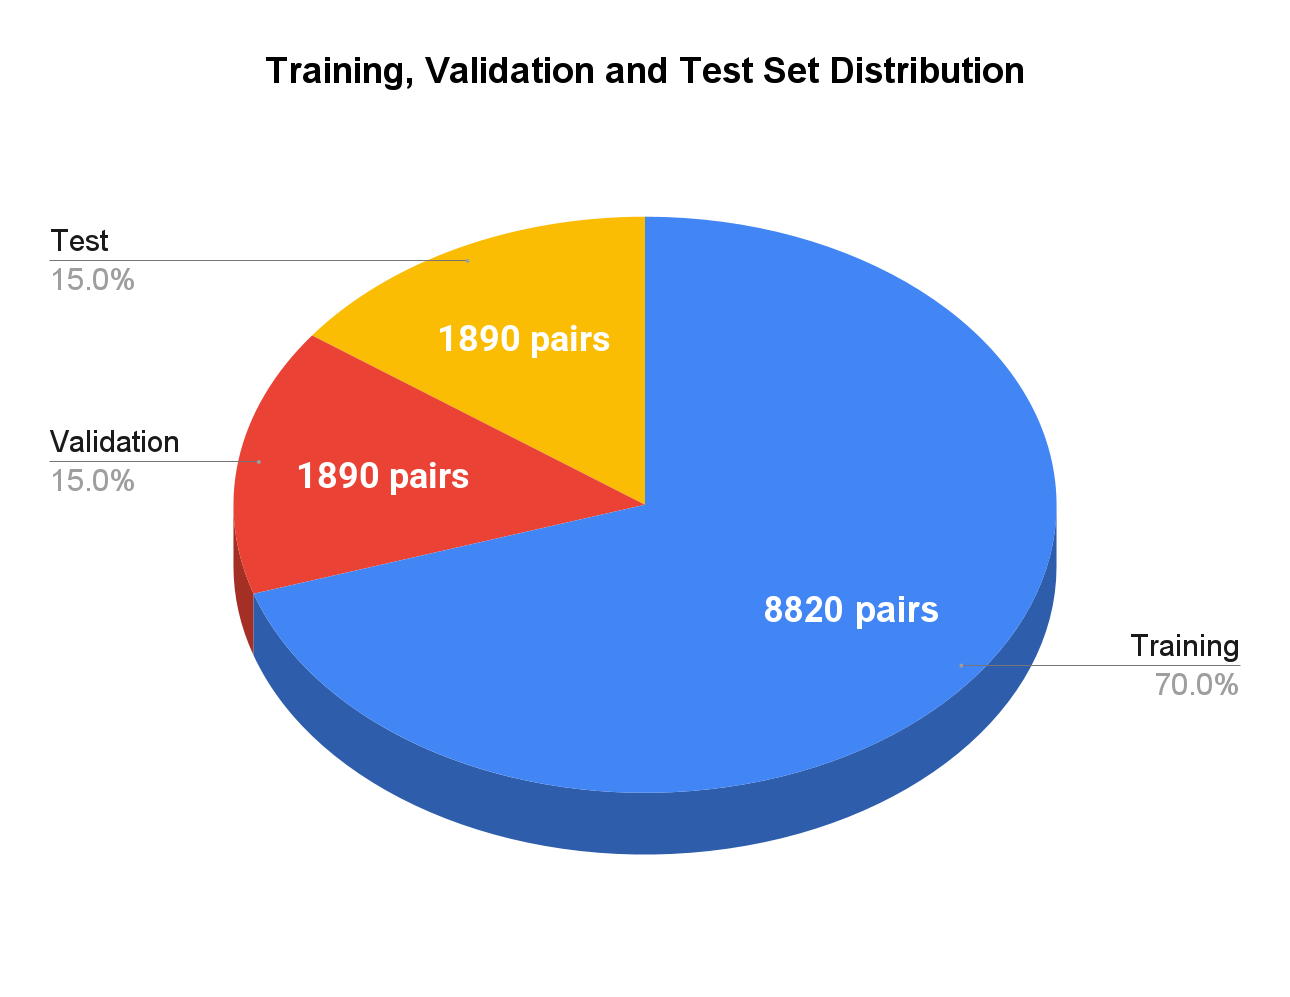
\includegraphics[width=0.65\linewidth]{Figs/dataset1.png}
  \caption{Training, Validation and Test Set Distribution of 12600 Image Pairs}
  \label{fig:dataset}
\end{figure}

\begin{figure}[htbp]            % h=here, t=top, b=bottom, p=page float
  \centering
  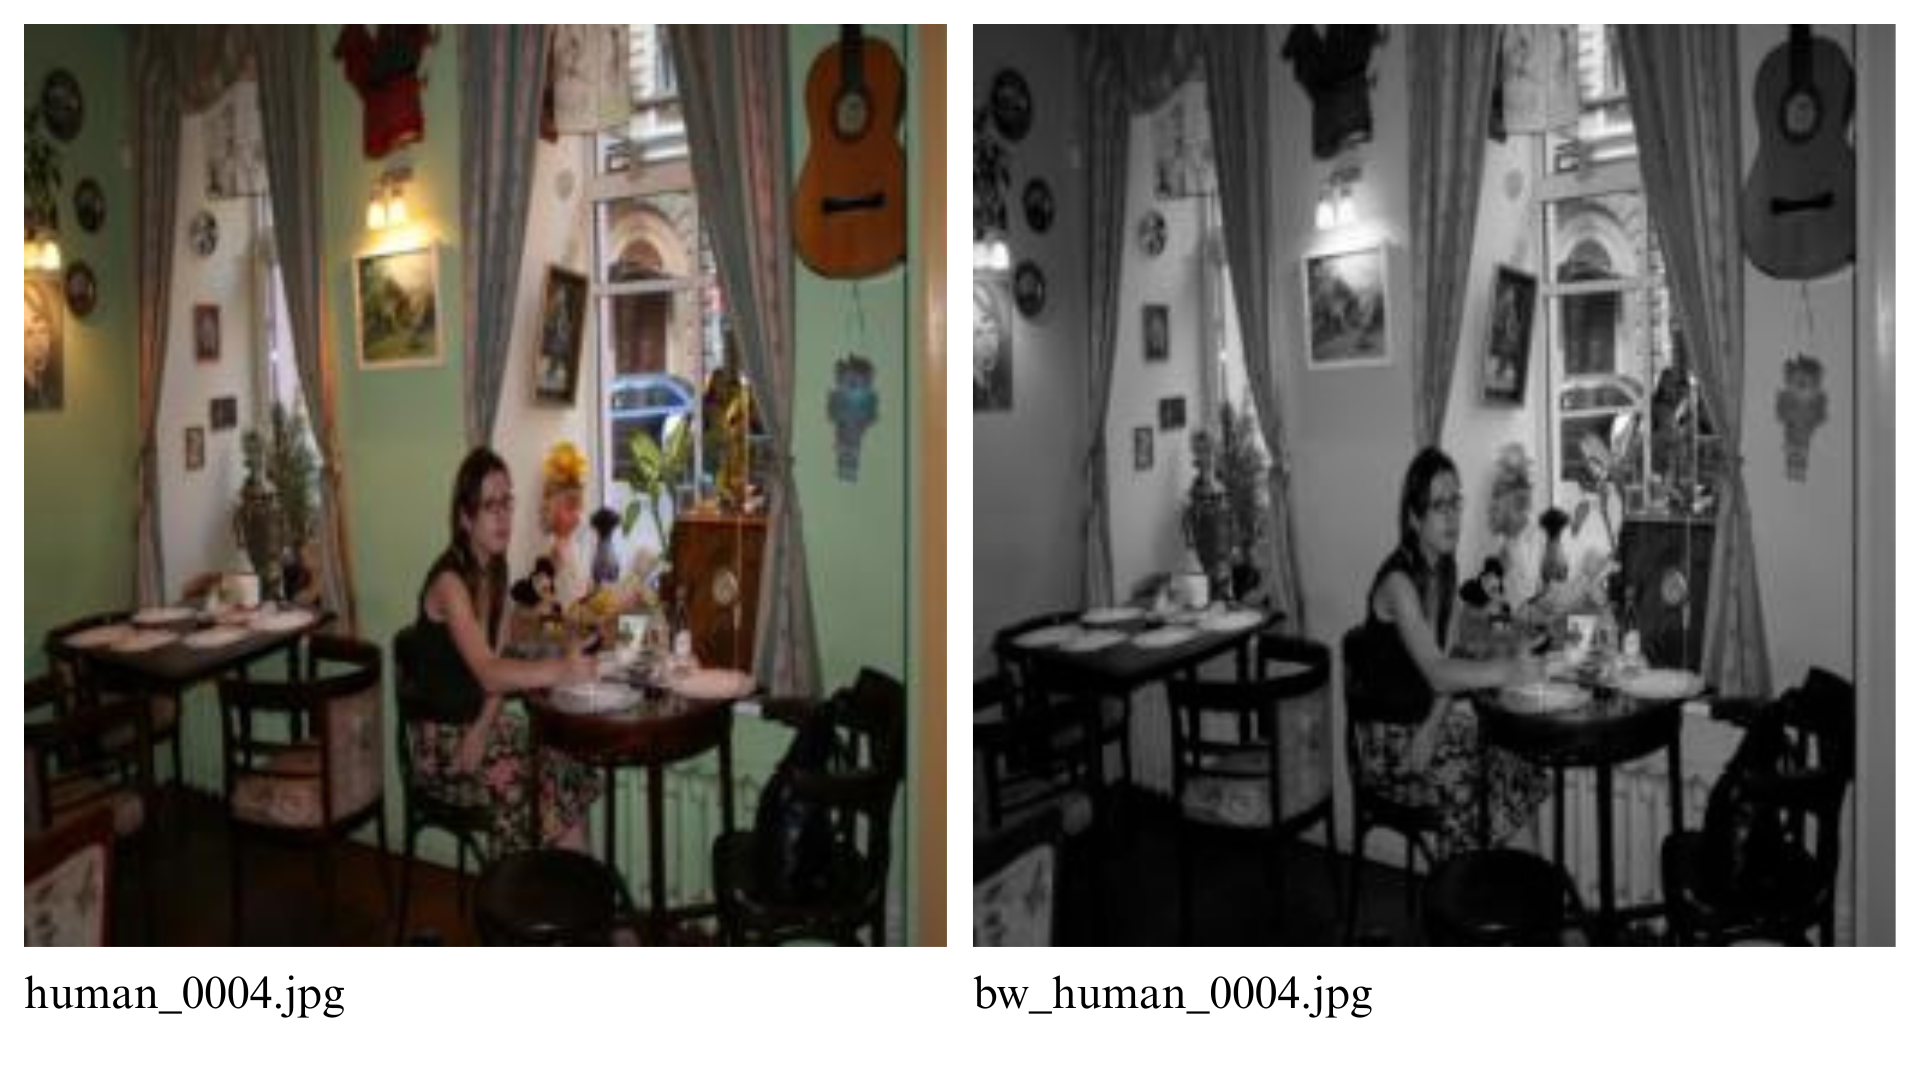
\includegraphics[width=0.65\linewidth]{Figs/Data Example.png}
  \caption{Sample Data Pair from Training Set}
  \label{fig:data_example}
\end{figure}

\subsection{Illustration}

\begin{figure}[htbp]            % h=here, t=top, b=bottom, p=page float
  \centering
  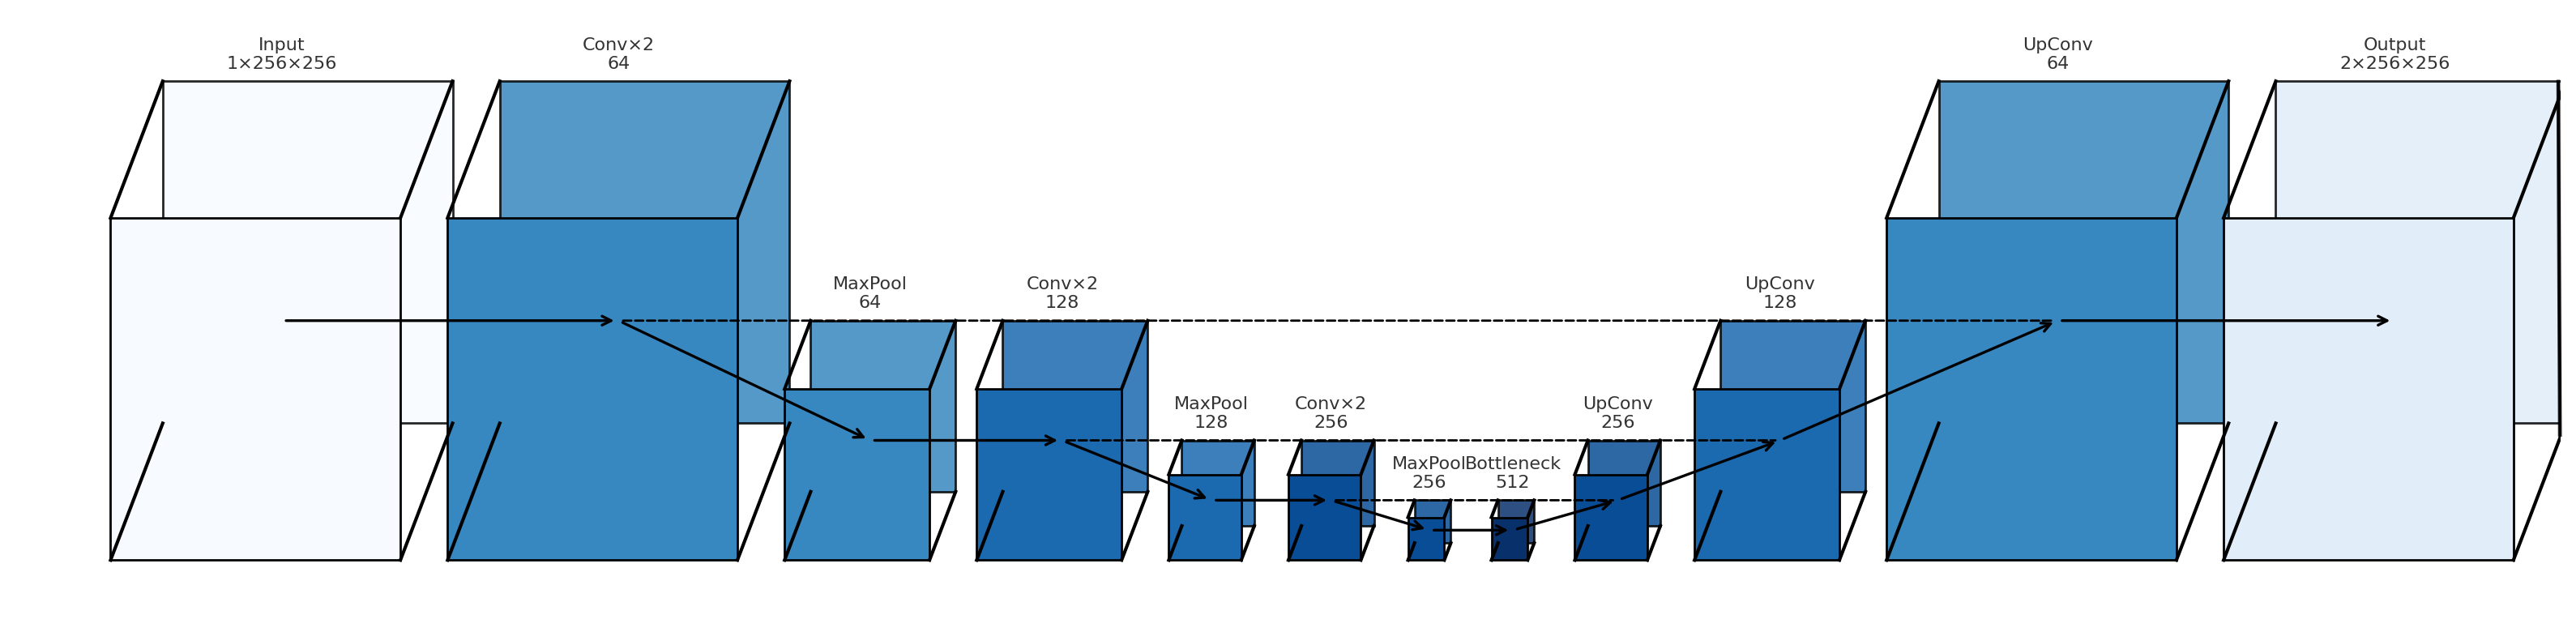
\includegraphics[width=0.9\linewidth]{Figs/architecture.png}
  \caption{Encoder–decoder colourization network with skip connections.}
  \label{fig:architecture}
\end{figure}

The top row is the encoder (Conv ×2 → MaxPool blocks) that downsamples the grayscale L channel from 256×256 to 32×32 while increasing feature depth (64 → 512).
The bottom row is the decoder (UpConv blocks) that upsamples back to full resolution and predicts the two chroma channels (a, b). Dashed arrows show the three skip connections that pass fine-grained features from encoder to decoder stages.

\subsection{Architecture}

We propose a convolutional encoder–decoder network for the colourization task, which is a common and effective choice for image-to-image translation problems. \cite{leatvanich2025image} The model will operate in the CIE Lab colour space: the input is a grayscale image (the L channel), and the network is trained to predict the two chrominance channels (a and b) as output. After prediction, the input L channel and the output a,b channels are combined and converted back to an RGB image for visualization. Using the Lab space decouples intensity from colour, which aligns with human vision and generally produces more realistic results than direct RGB prediction. \cite{leatvanich2025image}

The architecture itself is an encoder–decoder CNN resembling a simplified U-Net. The encoder consists of several convolutional layers (with ReLU activations and batch normalization) that gradually downsample the image, extracting higher-level features as the spatial size reduces. For example, we might start with a 3x3 conv layer with 64 filters, followed by another conv layer with 128 filters, each followed by a pooling (or stride-2 conv) to halve the spatial dimensions. After a few such layers, a bottleneck layer (e.g. a 3x3 conv with 256 filters) will capture abstract features of the grayscale input. The decoder then mirrors this process: it uses upsampling layers (e.g. Conv2DTranspose or nearest-neighbor upsampling) and additional conv layers to upsample the feature maps back to the original image resolution while predicting the a,b colour channels. We plan to include skip connections between matching encoder and decoder levels (as in U-Net) so that fine-grained details from early layers (edges, textures) are directly passed to the corresponding decoder layers. These skip connections should help the network recover details and prevent blurry outputs by combining low-level and high-level features. \cite{leatvanich2025image}

To balance performance and simplicity, we will leverage transfer learning for the encoder. In particular, we are considering initializing the encoder with a pretrained backbone like the first few layers of ResNet-18 or VGG16 (trained on ImageNet). This gives the model a head-start in recognizing semantic features—useful given our dataset of human and animal images, where recognizing objects like faces, fur, or backgrounds can inform colour choices. \cite{olah2022lettherebecolor} Using a pre-trained encoder should enable the network to learn meaningful colourization with fewer training examples and epochs. \cite{olah2022lettherebecolor} The decoder and any additional layers will be initialized randomly and learned from scratch. We will train the network end-to-end to minimize a pixel-wise loss between the predicted and ground-truth colour channels (e.g. mean squared error in Lab space).

It’s worth noting that some prior works frame colourization as a classification problem over discrete colour bins to better capture the ambiguous nature of predicting colour. For instance, Zhang et al. (2016) predict a probability distribution over possible a,b values for each pixel instead of regressing exact values. \cite{olah2022lettherebecolor} While such techniques (often coupled with class re-balancing or perceptual losses) can produce vibrant results, they add complexity beyond the scope of a course project. In our architecture, we favor a straightforward regression approach – the network directly outputs continuous a and b values – which is simpler to implement and sufficient for plausible colourization.

\subsection{Baseline Model}

As a baseline, we will start with a very simple colourization approach against which to compare our full model. One trivial baseline is to output the input grayscale image as-is in colour (i.e. replicate the L channel into RGB), which yields a degenerate colourization. This sets a minimum benchmark – any learning model should outperform simply producing a monochrome image.

For a more meaningful baseline, we will implement a shallow convolutional network inspired by basic encoder–decoder examples. \cite{leatvanich2025image} This baseline model will take the grayscale L channel as input and produce a,b chrominance channels, but it will have only a small fraction of the capacity of our main architecture. For instance, the baseline could use just two convolutional layers for encoding (e.g. 64 filters and 128 filters) followed by a single upsampling decoder to reconstruct the output colours. Concretely, the image might pass through Conv2D(64) and Conv2D(128) layers (with ReLU), then a pooling layer to downsample; at that point a minimal “bottleneck” conv layer can be applied, and finally an upsampling (Conv2DTranspose) step generates the 2-channel output map. \cite{leatvanich2025image} This simplistic model does not incorporate any skip connections or pretrained knowledge, and it has far fewer parameters than the proposed full model. We expect its predictions will capture only basic correlations (for example, mapping lightness to a bland average colour) and often look desaturated or unrealistic. \cite{rosebrock2019bwcolorization}

Such a baseline provides a useful point of comparison: it represents what a rudimentary learning method can achieve without much capacity or context. By evaluating our advanced model against this baseline, we can quantify the gains from using a deeper architecture and more sophisticated design. If the baseline’s output is dull or mostly grayish (as often seen in naive colourization attempts), whereas our full model produces more vibrant and context-appropriate colours, it will demonstrate the effectiveness of the chosen architecture. \cite{rosebrock2019bwcolorization}

\section{Ethical Considerations}
\label{ethical}

The dataset being used is public, so there are no copyright or consent issues. However, the dataset may contain racial or demographic imbalances, which could cause the model 
to generalize poorly or be biased towards specific skin tones. This may result in racially inaccurate or culturally insensitive outputs. A similar behaviour may be observed with 
animals, where a lack of diversity in breeds or fur colours in the dataset can result in misleading results. If the outputs produced by the model are used in educational contexts 
or in breed identification, they can contribute to misinformation. Furthermore, since the model results are plausible but cannot be verified, there is a risk that users may 
overtrust the outputs in sensitive contexts.

\section{Project Plan}
\label{project_plan}

Our high-level project planning has been completed using a Gantt chart (see Appendix A). It contains many of the detailed tasks we have completed and will complete in the future. This
easily shows who is responsible for each task, the time it will take to complete, and the dependencies between tasks. Generally, our internal deadlines have been set at least a 
few days prior to the official deadlines to ensure ample time to review our work and make necessary changes. In the event that a new member joins the team, they can easily
refer to this chart to see what responsibilites they can take on and what tasks are still available.

\subsection{Team Communication \& Coordination}

We intend to use Discord as our primary communication platorm, Google Drive for file sharing (Colab notebooks, datasets, etc.), and GitHub for version control. To ensure we do 
not overwrite each other's work, we will use branches for each feature or task, and merge them into the main branch once they are complete. We will also have weekly meetings to
discuss our progress, any issues we are facing, and plan for any action items for the subsequent meeting. Currently, we intend to meet on Saturday mornings at 8:00 AM EST as some
of our team members are in different time zones.

\section{Risk Register}
\label{risk_register}

This section outlines potential risks that may impact the progress or quality of the project, along with corresponding mitigation 
strategies. Identifying these risks early allows the team to plan contingencies and maintain project momentum even in the face 
of unforeseen challenges.

\subsection{Team Member(s) Drop Course}
If a team member drops the course or is unable to contribute due to illness or other unforeseen circumstances—especially close to a major 
deadline—we will revisit the Gantt chart to reallocate their tasks evenly among the remaining team members 
based on individual availability and strengths. Where necessary, we will reduce the scope of non-critical tasks to ensure that 
core deliverables are still completed on time. Regular check-ins and shared documentation will help ensure continuity.

\subsection{Model Training Taking Longer Than Expected}
Training time may exceed expectations due to hardware limitations, unexpected model complexity, or hyperparameter tuning. 
To mitigate this, we will build buffer time into our schedule to accommodate longer training runs. We will also regularly 
checkpoint models and keep logs for easy resumption. If training remains infeasible, we will simplify the architecture or 
reduce the dataset size without compromising class diversity, or shift to using cloud resources like Google Colab Pro if needed.

\subsection{Model Overfits to Stereotypical Colours}
Our model may learn biases from the dataset, such as assuming all skies are blue or all humans have certain skin tones. 
To mitigate this, we will include a validation set with diverse examples, use data augmentation (e.g., colour jitter, flipping), 
and regularly evaluate qualitative outputs—especially for edge cases. We will also explore loss terms or regularization 
strategies that discourage overconfident predictions. If overfitting persists, we may rebalance the dataset or adjust the 
loss function to reduce dependence on prior colour distributions.

\label{last_page}

\newpage
\bibliographystyle{iclr2022_conference}
\bibliography{APS360_ref}

\newpage
\section{Appendix A: Gantt Chart}
\begin{figure}[htbp]
  \centering
  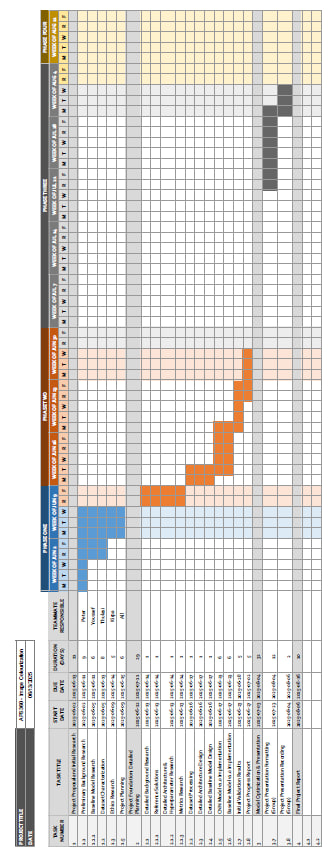
\includegraphics[width=0.55\linewidth]{Figs/gant-chart-full.jpg}
  \label{fig:gantt_chart}
\end{figure}
\end{document}
